\documentclass[12pt]{article}
\pagestyle{plain}
\usepackage{amsmath}
\usepackage{bm}
\usepackage{graphicx}
\graphicspath{ {./} }
\usepackage{float}

\begin{document}

\title{PhD Candidacy Exam Proposal:}
\author{c praise anyanwu \\
    Chemistry Department, University of Washington
    \thanks{anyanc@uw.edu} }
\date{14 September 2022}
\maketitle

\newpage
\section{A Single Photon Source Enabled by Fano Interference between a
Broadband Emitter and a High Q, Kerr Cavity}

\subsection{Introduction}
Single photon sources play a prominent role in the field of quantum information 
science. \cite{gisin2002quantum, bennett2004quantum} In the QKD protocol, Alice encodes 
an information, for example, in the quibit of a photon polarization state. If Alice must 
securely transmit this quibit through a quantum channel to Bob, the reciever, then 
Alice's single photon source must be deterministic. In a case where Alice generates a 
probalistic two-photon state, then Eve, the eavesdropper, can glean information from one 
of the two photons (unbeknownst to Alice) while the second photon is transmitted to Bob. 
\cite{bennett1984proceedings, bennett1992quantum} Moreover, since photons travel at the 
speed of light and interact weakly with the environment over long distances, enconding 
infromation in the quanutm state of a single photon (using degrees of freedom of 
polarization, momentum, or energy) is hihgly compatible and thus desirable in 
quantum communication application.

A deterministic single-photon source that emits a single photon \textit{on demand}, 
with $100 \: \%$ probability, is ideal. In practice, one evaluates the 
single-photon nature of a source by the ratio of the probability of single-photon 
to multi-photon emission, and thus single-photon sources lie on a spectrum of 
two main classes: deterministic and probabilistic sources. \cite{lounis2005single, 
eisaman2011invited} The former involves effective two level systems (quantum
dots, single atoms, single ions) \cite{ShieldsAndrewJ2007Sqls, strauf2007high, 
hennrich2004photon, wilk2007single, maurer2004single} that emit a single photon when 
excited by a resonant incident field; the latter involves, for example, parametric 
down conversion in waveguides (or four-wave mixing in optical fiber) systems
\cite{u2004efficient, sharping2001observation, goldschmidt2008spectrally} 
that emit a correlated pair of photons, where one photon heralds the other. 
The known difficulties with these systems involve trapping of a single ion or atom 
strongly coupled to cavities at cryogenic temperatures for deterministic single-photon 
sources, and care must be taken with the probabilistic sources to avoid generating 
multiple pairs of photons. Herein, we propose a theoretical basis for a novel system that 
circumvents ion trapping at ultra-cold temperatures, and this system is operative in the 
Purcell regime; then we calculate the second order correlation function as a measure of 
its single-photon nature.

\begin{figure}[H]
  \centering
  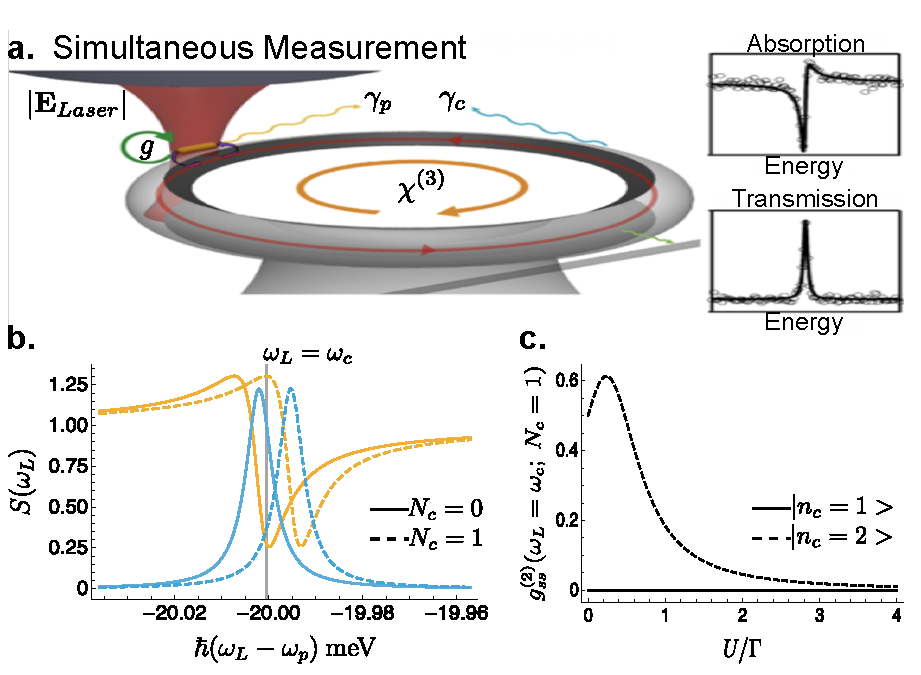
\includegraphics[width=1\linewidth]{fig.pdf}
  \caption{(a) Example of the proposed experimental set-up
  \cite{pan2019elucidating}, which in general, consists of a broad-band
  quantum emitter (here represented as gold nanorod) placed unto\textemdash
  and weakly coupled to\textemdash a kerr-cavity (here represented as
  toroidal micro-ring resonator). The emitter is pumped with a
  Laser, and its absorption spectrum shows a Fano profile due
  to its interaction with the High-Q cavity. At the vicinity of the
  anit-resonance, there is a peak in tramission of light through the cavity
  out-coupled to the measuring fiber optic cable. (b) The spectral distribution
  of the reduced average photon-number in the broad-band mode at steady-state
  $<\hat{b}^{\dagger}\hat{b}>_{ss}/<\hat{b}^{\dagger}\hat{b}>_{ss; g=0}$,
  yellow curves, and the average photon number in the discrete cavity mode of a
  single-photon state $<n_c=1|\: \hat{a}^{\dagger}\hat{a} \: |n_c=1>_{ss}$, 
  blue curves. The solid curves are the spectra when the cavity has zero-photon
  occupation $N_c=0$, while the dashed curves, the cavity has a single-photon
  occupation $N_c=1$. (c) The second order correlation calculated at steady
  state when the cavity is populated with a single-photon occupation.
  The single-photon blockade is eviedent for a kerr-nonlinearity whose value is
  withtin the order of the Fano line-width, i.e., $U=\Gamma$.
  }
  \label{fig}
\end{figure}

Consider the following system: a high-quality cavity coupled to a broadband emitter. 
For example, ref \cite{pan2019elucidating} has a near sub-diffraction plasmon nanorod 
placed on the chip of a torodial silicon based microcavity, with a $10^{7}$ Q-factor. 
The absorbtion crossection of the excited plasmon nanorod yields a Fano-lineshape slighly 
shifted about the resonace of the isolated mode of the microcavity. This Fano resonance 
is indicative of a hybrid mode of the hybridized plasmonic-photonic system. Moreover, 
not only is this system operative at room temperature, it is capable of measuring 
attometer shifts in the resonances of the microcavity modes. We propose the following 
modification: coating the cavity with polystyrene, which has a large third-order nonlinear susceptibility on the order of $10^{−12} \:\mathrm{cm}^2/\mathrm{W}$. 
\cite{qin2010design, liu200910}. (Polystyrene's third-order nonlinearity originates 
from the delocalization of the $\pi$-conjugated electrons along the polymer chains. 
\cite{krausz1989optical, wong1991studies}) This achieves a kerr effect such that 
transmission of a photon from the pump laser (through the plasmon) to the cavity would 
result in the shift of the cavity's resonance (see figure). Thus the resonance of the 
nonlinear cavity now depends on the photon-number in the cavity.

A characteristic of this nonlinear plasmonic-photonic system is the cavity photon-number 
dependent Fano resonance, with a sharp resonant peak and anti-resonant dip corresponding 
to an enhanced and diminished plasmon absorption cross-section (see figure). At the 
anti-resonant frequency of diminished plasmon absorption, there is a transmision of 
photon into the cavity. Thus, a pump laser exciting the plasmon at the anti-resonance 
would yield, ideally, a single-photon occupation in the cavity; and for a non-linear 
cavity, this single-photon occupation would result to a shift of the Fano resonance
(see yellow curve of figure). If this shifted Fano resonance (of the cavity mode with 
a single-photon occupation) now yields a peak of enhanced plasmon absorption that aligns 
with the pump laser, then any subsequent photon will be absorped by the plasmon. Thus, 
the system exhibits a blockade effect for a two-photon transition at the resonant peak
aligned with the pump laser, however, permiting a single-photon transition at the 
anti-resonant dip aligned with the pump laser. We set out to calculate the second order 
correlation function of such single- and two-photon states of the proposed nonlinear 
cavity-emitter system.

We develop the system's dynamics in Heisenberg picture. Heisenberg picture is 
suitable to calculate the quantum statistical correlation of the field of light 
transmitted throught the kerr cavity. This field correlation can be related to 
the experimentally observed spectral distribution, using the spectral response 
function. \cite{scully1999quantum} Moreover, in the Heisenberg picture the 
dynamics of the quantum transverse field is analogous to the classical 
transverse field \cite{tannoudji1992atom}, which allows for direct comparison 
to the classical system. \cite{pan2019elucidating} Then damping of the 
single-mode in the cavity field (and of the broad-band field) is described 
using Heisenberg-Langevin formalism. In so doing, this model provides a simple 
yet rigorous quantum approach (complementing the Louivillian formalism in the
Linblad form, recently developed in Ref. \cite{finkelstein2015fano, 
finkelstein2016nonlinear}) to account for damping of the discrete state 
(cavity mode) of Fano resonance, and the spectral distribution derived from 
this model is expressed in terms of Fano-parameters. \cite{fano1961effects}


\subsection{Model}
The Hamiltonian of the discrete kerr-cavity coupled to a broad-band emitter is
the following $\mathcal{H} = \mathcal{H}_{a} + \mathcal{H}_{b} + 
\mathcal{H}_{f} + \mathcal{H}_{I}$. The derived Hamiltonian $\mathcal{H}_{a}$ 
is the energy of a single-mode dielectric kerr-cavity in free space 
\cite{jackson1999classical}, such that,
\begin{equation}
\begin{split}
\mathcal{H}_{a} &= \frac{1}{2} 
    \int_{V} \mathrm{d}^{3}\mathbf{x} \: \mathbf{P} \cdot \mathbf{E}
\\
&= \frac{1}{2} 
    \int_{V} \: \mathrm{d}^{3}\mathbf{x}
    \Big( \mathbf{P}^{(1)} + \mathbf{P}^{(3)} \Big)
    \cdot \mathbf{E}
\\
&= \frac{1}{2} 
    \int_{V} \: \mathrm{d}^{3}\mathbf{x} \: 4\pi 
    \Big( \bm\chi^{(1)} \mathbf{E}  + 
    \frac{3}{4}\bm\chi^{(3)}:\mathbf{E}\mathbf{E}^{*} \mathbf{E} \Big)
    \cdot \mathbf{E}
\end{split}
\end{equation}
where $3/4\mathbf{\chi}^{(3)}$ is the higher order non-linear suceptibility of
a kerr-cavity \cite{butcher1990elements}, and the quantized field $\mathbf{E}$
is normalized with respect to the cavity's mode volume $V$. In the rotating
wave approximation (and for a linear polarization), $\mathcal{H}_{a}$
simplifies as follows
\begin{equation}
\begin{split}
\mathcal{H}_{a} &= \hbar\omega_k 4\pi^{2} \Big(
    \chi^{(1)}_{ef} +
    \frac{3}{4} \chi^{(3)}_{ef} \mathcal{E}^2
    a^{\dagger}a + \frac{3}{4}\bm\chi^{(3)} \mathcal{E}^2 : \mathbf{1} \Big)
    \Big( a^{\dagger}a + \frac{1}{2} \Big)
\\
&= \hbar \Big( \omega_c + U\:a^{\dagger}a \Big)
    \Big( a^{\dagger}a + \frac{1}{2} \Big)
\\  
&\approx \hbar \Big( \omega_c + U \langle a^{\dagger}a \rangle \Big)
    \Big( a^{\dagger}a + \frac{1}{2} \Big).
\end{split}
\end{equation}
where $\mathcal{E} = \sqrt{2\pi \hbar \omega_k / V }$ is the amplitude of the
quantized field.

The first-order approximation in Eq. (5) linearizes the non-linear term.
This is based on the motivation that the resonant frequency of a kerr-cavity
changes as a function of intesity $|\mathbf{E}|^2$. In this case, the resonant
frequency depends on the average photon-number in the kerr-cavity
\begin{equation}
\omega_c^{NL}( N_c = \langle a^{\dagger}a \rangle )  = \omega_c + UN_c.
\end{equation}
Thus the Hamilonian for the single-mode kerr-cavity $\mathcal{H}_a$, the 
bosonic broad-band field $\mathcal{H}_b$, and the free field $\mathcal{H}_f$
is as follows
\begin{align}
\mathcal{H}_a &= \hbar\omega_c^{NL}
    \Big( a^{\dagger}a + \frac{1}{2} \Big),
\\
\mathcal{H}_b &= \hbar\omega_p
    \Big( b^{\dagger}b + \frac{1}{2} \Big),
\\
\mathcal{H}_f &= \hbar \sum_j \omega_j
    \Big( f^{\dagger}_j f_j + \frac{1}{2} \Big),
\end{align}
The discrete cavity mode $\omega_c^{NL}$ and the broad-band mode $\omega_p$
both disipate energy to the free fields $\omega_k$. Thus the interaction
Hamiltonian $\mathcal{H}_{I}$ is as follows
\begin{equation}
\mathcal{H}_I = \hbar g \: (
    a^{\dagger}b + b^{\dagger}a )
    + \hbar \sum_j ( V_j^a f^{\dagger}_j a 
        + V_j^b f^{\dagger}_j b + \mathrm{h.c.} ).
\end{equation}
We work in the purcell regime where $|V_a| \ll g \ll |V_b|$. Note that the
original Fano problem is the limit where $|V_a| \rightarrow 0$.

Deriving the Heisenberg-Langevin equation of motion for the slowly varying
operator $A = a \: e^{i\omega_c^{NL} t}$, and then 
transforming back to the non-slowly varying operator $ a = 
A \: e^{-i\omega_c^{NL} t}$ yields
\begin{align}
\dot{ a } &= -i ( \omega_c^{NL} - i\gamma_c/2 ) a 
    - ig b,
\\
\dot{b} &= -i ( \omega_p - i\gamma_p/2 ) b
    - ig a,
\end{align}
$\gamma_{c,p}$ accounts for both radiative and non-radiative damping as
described in Ref \cite{thakkar2015quantum}. (Note that the above equation
has assumed an evacuated initail reservoir state.)

In the experiment, the broad-band mode is driven by the external
field of a monochromatic laser operating at $\omega$. The spectral 
distribution is derived from the spectral response function, such that,
\begin{equation}
S(\omega) = \frac{1}{\pi} \int_0^{\infty} \mathrm{d}\tau \: 
    e^{i \omega \tau} 
    \langle b^{\dagger}(t_0=0) \: b(t_0 + \tau) \rangle.
\end{equation}
We find that the spectral reponse function can be interpreted as the steady 
state solution of the average photon-number in the broad-band mode rotating 
in the frame of a drive frequency, i.e.
\begin{align}
S(\omega) &= \langle \tilde{b}^{\dagger}_{ss}\tilde{b}_{ss} \rangle
\\
\tilde{b}^{\dagger}_{ss} &= 
    b^{\dagger}_{ss} \: e^{i \omega_L t}; \quad
    \tilde{a}^{\dagger}_{ss} =
    a^{\dagger}_{ss} \: e^{i \omega_L t};
\\
\dot{b}_{ss} &= 0 =
    -i ( \omega_p - i\gamma_p/2 ) b_{ss} - ig a_{ss}
    + iE_{drive}( e^{i \omega_L t} - e^{-i \omega_L t} ).
\end{align}
and $E_{drive}$ is the amplitude of the monochromatic laser operating at
a drive frequency $\omega = \omega_L$. The reduced spectral response yields
\begin{equation}
\begin{split}
\frac{ S(\omega = \omega_L) }{ S(\omega = \omega_L)_{g=0} } &= 
    \frac{\langle \tilde{b}^{\dagger}_{ss}\tilde{b}_{ss} \rangle}
        {\langle \tilde{b}^{\dagger}_{ss}\tilde{b}_{ss} \rangle}_{g=0}
\\
&= \Bigg( 1 +
    \frac{\gamma_c}{\gamma_p}
    \frac{g^2}{(\omega_L - \omega_c^{NL})^2 + (\gamma_c/2)^2}
    \Bigg) \:
    \left\vert \frac{q + \epsilon}{\epsilon + i} \right\vert.
\end{split}
\end{equation}
The first term is the Fano profile, where 
$\epsilon=(\omega_L - \omega_{eff})/(\gamma_{eff}/2)$ and 
$q = (\omega_c^{NL} - i\gamma_c/2 - \omega_{eff})/(\gamma_{eff}/2)$;
$\omega_{eff}$, $\gamma_{eff}$, and $q$ are the Fano parameters. The second
term is the Lorentz distribution due to the line-width broadening of the
discrete state. The spectral distribution reduces to the Fano profile in the
limit $\gamma_c \propto |V_a| \rightarrow 0$.

Since we are interested in single-photon blockade due to the kerr 
non-linearity, $U \propto \chi_{eff}^{(3)}$, we calculate the second order
correlation function $g^{(2)}$ of light transmitted through the kerr-cavity
coupled to the driven broad-band emitter, at the steady state, as a function
of U, i.e.,
\begin{equation}
\begin{split}
g^{(2)}_{ss}(U) &\equiv 
    \frac{ \langle n_a, n_b \vert \:
    \tilde{a}^{\dagger}_0 \: \tilde{a}^{\dagger}_{ss}(U)
    \tilde{a}_{ss}(U) \: \tilde{a}_0 \:
    \vert n_a, n_b \rangle }
    {(\langle \tilde{a}^{\dagger}_0\tilde{a}_0 \rangle)^2}
\\
&= \frac{n_a \langle n_a - 1, n_b \vert \:
    \tilde{a}^{\dagger}_{ss}\tilde{a}_{ss} \:
    \vert n_a - 1, n_b \rangle}
    {n_a^2}
\\
&= \frac{1}{n_a} 
    \frac{g^2}
    {\left\vert \omega_L - \omega_c^{NL}(U) + i\gamma_c/2 \right\vert^2}
    \langle n_a - 1, n_b \vert \:
    \tilde{b}^{\dagger}_{ss}\tilde{b}_{ss} \:
    \vert n_a - 1, n_b \rangle
\\
&= \frac{g^2}{n_a}
    \frac{\langle n_a-1 \vert \: E_{Laser}^2 \: \vert n_a-1 \rangle}
    {\left\vert \big( \omega_L - \omega_c^{NL}(U) + i\gamma_c/2 \big)
    \big( \omega_L - \omega_p + i\gamma_p/2 \big)
    -g^2 \right\vert^2}.
\end{split}
\end{equation}
For single-photon blockade, the photon-number in the cavity is set to one,
such that, $\omega_c^{NL}( N_c = 1 )  = \omega_c + U$. Importantly, the
amplitude of the Laser field to populate the bare ($N_c=0$) cavity mode 
with a single photon at steady state is such that
\begin{equation}
\begin{split}
\langle n_a=1 \vert \:
    \tilde{a}^{\dagger}_{ss} \tilde{a}_{ss} \:
    \vert n_a=1 \rangle 
    &= n_a = 1
\\
&= \frac{ g^2 \: 
    \langle n_a \vert \: E_{Laser}^2 \: \vert n_a \rangle}
    {\left\vert \big( \omega_L - \omega_c^{NL}(N_c=0) + i\gamma_c/2 \big)
    \big( \omega_L - \omega_p + i\gamma_p/2 \big)
    -g^2 \right\vert^2}.
\end{split}
\end{equation}
thus, it follows that
\begin{equation}
\langle n_a \vert \: E_{Laser}^2 \: \vert n_a \rangle = n_a
    \left\vert 
    ( i\gamma_c/2 )( \omega_c - \omega_p + i\gamma_p/2 ) -g^2 
    \right\vert
    / g.
\end{equation}


\subsection{Analysis}
The two-photon blockade effect depends on the Fano resonance shift induced by the kerr 
cavity. The system is designed such that a monochromatic pump laser aligns with the 
anti-resonant frequency (corresponding to a diminished plasmon absorption) of a 
single-photon transition but aligns with the resonat frequency (corresponding to an 
enhanced plasmon absorption) of a two-photon transition; the former state transmits into 
the cavity while latter state is absorped by the plasmon. Thus the degree of nonlinearity 
depends on the line-width between the anti-resonant dip and the resonant peak of the 
Fano line-shape, such that,
\begin{equation}
\begin{split}
\lambda_1 - \lambda_2 &= \lambda_1 - (\lambda_1 + 2\pi c / \Gamma )
\\
\Delta\lambda &= 2\pi c / \Gamma
\end{split}
\end{equation}
where $\Gamma$, the FWHM, is approximately equal to the line-width between the 
anti-resonant dip and the resonant peak of the Fano-lineshape; $\lambda_1$ and 
$\lambda_2$ are the wavelengths of the modes associated with the single- and two-photon
transitions, respectively.  Assuming the whispering-gallery modes of the torodial 
kerr-cavity as standing waves, then $\lambda_{1,2}/n_{1,2} = 2L/m$, where $n_2$
is the refractive index of the kerr-cavity \cite{spillane2002ultralow}:
\begin{equation}
\begin{split}
n_2 &= n_1 + \Delta n I
\\
&= n_1 + \frac{3 \chi^{(3)}}{8 n_1 c\epsilon_0} I.
\end{split}
\end{equation}

The kerr effect is induced by the local intensity $I$ from the pump laser populating
the kerr-cavity. From the above equations we find the relation:
\begin{equation}
\begin{split}
\frac{\Delta \lambda}{\lambda_1 / n_1} &= \Delta n I \\
&= \frac{3 \chi^{(3)}}{8 n_1 c\epsilon_0} I
\end{split}
\end{equation}
For a pump laser operating at an intensity $\approx 80 \:\mathrm{GW/cm^{2}}$, with 
a third order susceptibility $\approx 1.15 \times 10^{-12} \:\mathrm{cm}^2/\mathrm{W}$, 
\cite{qin2010design} and for a cavity mode $\lambda_{1}/{n_1} \approx 1550 \:\mathrm{nm}$, the desired blockade effect can be achieved for a two-photon state whose resonance is 
shifted by $\Delta\lambda \approx $. This value serves as an upper bound since the 
fano-lineshape has a narrow line-width on the order of an attometer. This is advantageous
because the desired blockade effect could be achieved for a kerr-cavity with a much 
smaller third order suceptibily and a faint laser beam (whose coherent state could have 
an average photon-number in the range $\mu = 1-4$).


\newpage
\bibliography{ref_database}
\bibliographystyle{unsrt}

\end{document}
